% Created 2023-01-20 fr 17:31
% Intended LaTeX compiler: pdflatex
\documentclass[12pt]{article}

%%%% settings when exporting code %%%% 

\usepackage{listings}
\lstdefinestyle{code-small}{
backgroundcolor=\color{white}, % background color for the code block
basicstyle=\ttfamily\small, % font used to display the code
commentstyle=\color[rgb]{0.5,0,0.5}, % color used to display comments in the code
keywordstyle=\color{black}, % color used to highlight certain words in the code
numberstyle=\ttfamily\tiny\color{gray}, % color used to display the line numbers
rulecolor=\color{black}, % color of the frame
stringstyle=\color[rgb]{0,.5,0},  % color used to display strings in the code
breakatwhitespace=false, % sets if automatic breaks should only happen at whitespace
breaklines=true, % sets automatic line breaking
columns=fullflexible,
frame=single, % adds a frame around the code (non,leftline,topline,bottomline,lines,single,shadowbox)
keepspaces=true, % % keeps spaces in text, useful for keeping indentation of code
literate={~}{$\sim$}{1}, % symbol properly display via latex
numbers=none, % where to put the line-numbers; possible values are (none, left, right)
numbersep=10pt, % how far the line-numbers are from the code
showspaces=false,
showstringspaces=false,
stepnumber=1, % the step between two line-numbers. If it's 1, each line will be numbered
tabsize=1,
xleftmargin=0cm,
emph={anova,apply,class,coef,colnames,colNames,colSums,dim,dcast,for,ggplot,head,if,ifelse,is.na,lapply,list.files,library,logLik,melt,plot,require,rowSums,sapply,setcolorder,setkey,str,summary,tapply},
aboveskip = \medskipamount, % define the space above displayed listings.
belowskip = \medskipamount, % define the space above displayed listings.
lineskip = 0pt} % specifies additional space between lines in listings
\lstset{style=code-small}
%%%% packages %%%%%

\usepackage[utf8]{inputenc}
\usepackage[T1]{fontenc}
\usepackage{lmodern}
\usepackage{textcomp}
\usepackage{color}
\usepackage{graphicx}
\usepackage{grffile}
\usepackage{wrapfig}
\usepackage{rotating}
\usepackage{longtable}
\usepackage{multirow}
\usepackage{multicol}
\usepackage{changes}
\usepackage{pdflscape}
\usepackage{geometry}
\usepackage[normalem]{ulem}
\usepackage{amssymb}
\usepackage{amsmath}
\usepackage{amsfonts}
\usepackage{dsfont}
\usepackage{array}
\usepackage{ifthen}
\usepackage{hyperref}
\usepackage{natbib}
%
%%%% specifications %%%%
%
\usepackage{ifthen}
\usepackage{xifthen}
\usepackage{xargs}
\usepackage{xspace}
\newcommand\Rlogo{\textbf{\textsf{R}}\xspace} %
\RequirePackage{fancyvrb}
\DefineVerbatimEnvironment{verbatim}{Verbatim}{fontsize=\small,formatcom = {\color[rgb]{0.5,0,0}}}
\RequirePackage{colortbl} % arrayrulecolor to mix colors
\RequirePackage{setspace} % to modify the space between lines - incompatible with footnote in beamer
\renewcommand{\baselinestretch}{1.1}
\geometry{top=1cm}
\RequirePackage{changepage}
\RequirePackage{colortbl} % arrayrulecolor to mix colors
\RequirePackage{pifont}
\RequirePackage{relsize}
\newcommand{\Cross}{{\raisebox{-0.5ex}%
{\relsize{1.5}\ding{56}}}\hspace{1pt} }
\newcommand{\Valid}{{\raisebox{-0.5ex}%
{\relsize{1.5}\ding{52}}}\hspace{1pt} }
\newcommand{\CrossR}{ \textcolor{red}{\Cross} }
\newcommand{\ValidV}{ \textcolor{green}{\Valid} }
\usepackage{stackengine}
\usepackage{scalerel}
\newcommand\Warning[1][3ex]{%
\renewcommand\stacktype{L}%
\scaleto{\stackon[1.3pt]{\color{red}$\triangle$}{\tiny\bfseries !}}{#1}%
\xspace
}
\hypersetup{
citecolor=[rgb]{0,0.5,0},
urlcolor=[rgb]{0,0,0.5},
linkcolor=[rgb]{0,0,0.5},
}
\RequirePackage{epstopdf} % to be able to convert .eps to .pdf image files
\RequirePackage{capt-of} %
\RequirePackage{caption} % newlines in graphics
\RequirePackage{enumitem} % to be able to convert .eps to .pdf image files
\definecolor{light}{rgb}{1, 1, 0.9}
\definecolor{lightred}{rgb}{1.0, 0.7, 0.7}
\definecolor{lightblue}{rgb}{0.0, 0.8, 0.8}
\newcommand{\darkblue}{blue!80!black}
\newcommand{\darkgreen}{green!50!black}
\newcommand{\darkred}{red!50!black}
\usepackage{mdframed}
\newcommand{\first}{1\textsuperscript{st} }
\newcommand{\second}{2\textsuperscript{nd} }
\newcommand{\third}{3\textsuperscript{rd} }
\date{\today}
\title{Results simulation study DelayedGSD}
\hypersetup{
 colorlinks=true,
 pdfauthor={},
 pdftitle={Results simulation study DelayedGSD},
 pdfkeywords={},
 pdfsubject={},
 pdfcreator={Emacs 27.2 (Org mode 9.5.2)},
 pdflang={English}
 }
\begin{document}

\maketitle

\section{Rejection rate}
\label{sec:org9d1a00c}

Power by method (columns) and scenario (rows): \hfill (nominal level 0.8)
\begin{verbatim}
 scenario     N missing binding  fixC ar method 1 method 2 method 3
        1 10000    TRUE    TRUE FALSE 10    81.00    80.79    80.45
        3 10000    TRUE    TRUE FALSE  5    80.60    80.45    80.21
        5 10000    TRUE    TRUE  TRUE 10    79.81    80.41    80.39
        7 10000    TRUE    TRUE  TRUE  5    80.00    80.46    80.08
        9 10000    TRUE   FALSE  TRUE 10    80.50    80.85    80.91
       11 10000    TRUE   FALSE  TRUE  5    80.73    80.82    80.75
       13 10000    TRUE   FALSE FALSE 10    80.67    80.60    80.65
       15 10000    TRUE   FALSE FALSE  5    80.65    80.64    80.46
       17 10000   FALSE    TRUE FALSE  5    80.31    80.28    79.93
\end{verbatim}
\Warning slightly too high power for some scenario

\bigskip

Type 1 error by method (columns) and scenario (rows): \hfill (nominal level 0.025)
\lstset{language=r,label= ,caption= ,captionpos=b,numbers=none}
\begin{lstlisting}
tablePrintH0 <- dcast(res2stageS.rejection[hypo=="typeI"],
                    scenario + N + missing + binding + fixC + ar ~ method.char,
                    value.var = "rejectionRate")
print(tablePrintH0, row.names = FALSE)
\end{lstlisting}

\begin{verbatim}
 scenario     N missing binding  fixC ar method 1 method 2 method 3
        2 10000    TRUE    TRUE FALSE 10     2.46     2.53     2.40
        4 10000    TRUE    TRUE FALSE  5     2.42     2.41     2.40
        6 10000    TRUE    TRUE  TRUE 10     2.25     2.25     2.45
        8 10000    TRUE    TRUE  TRUE  5     2.42     2.39     2.50
       10 10000    TRUE   FALSE  TRUE 10     2.09     2.09     2.26
       12 10000    TRUE   FALSE  TRUE  5     2.30     2.28     2.33
       14 10000    TRUE   FALSE FALSE 10     2.29     2.28     2.46
       16 10000    TRUE   FALSE FALSE  5     2.38     2.37     2.46
       18 10000   FALSE    TRUE FALSE  5     2.46     2.44     2.45
\end{verbatim}
\Warning slightly too lower type 1 error for some scenario

\clearpage

\begin{figure}[!h]
\centering
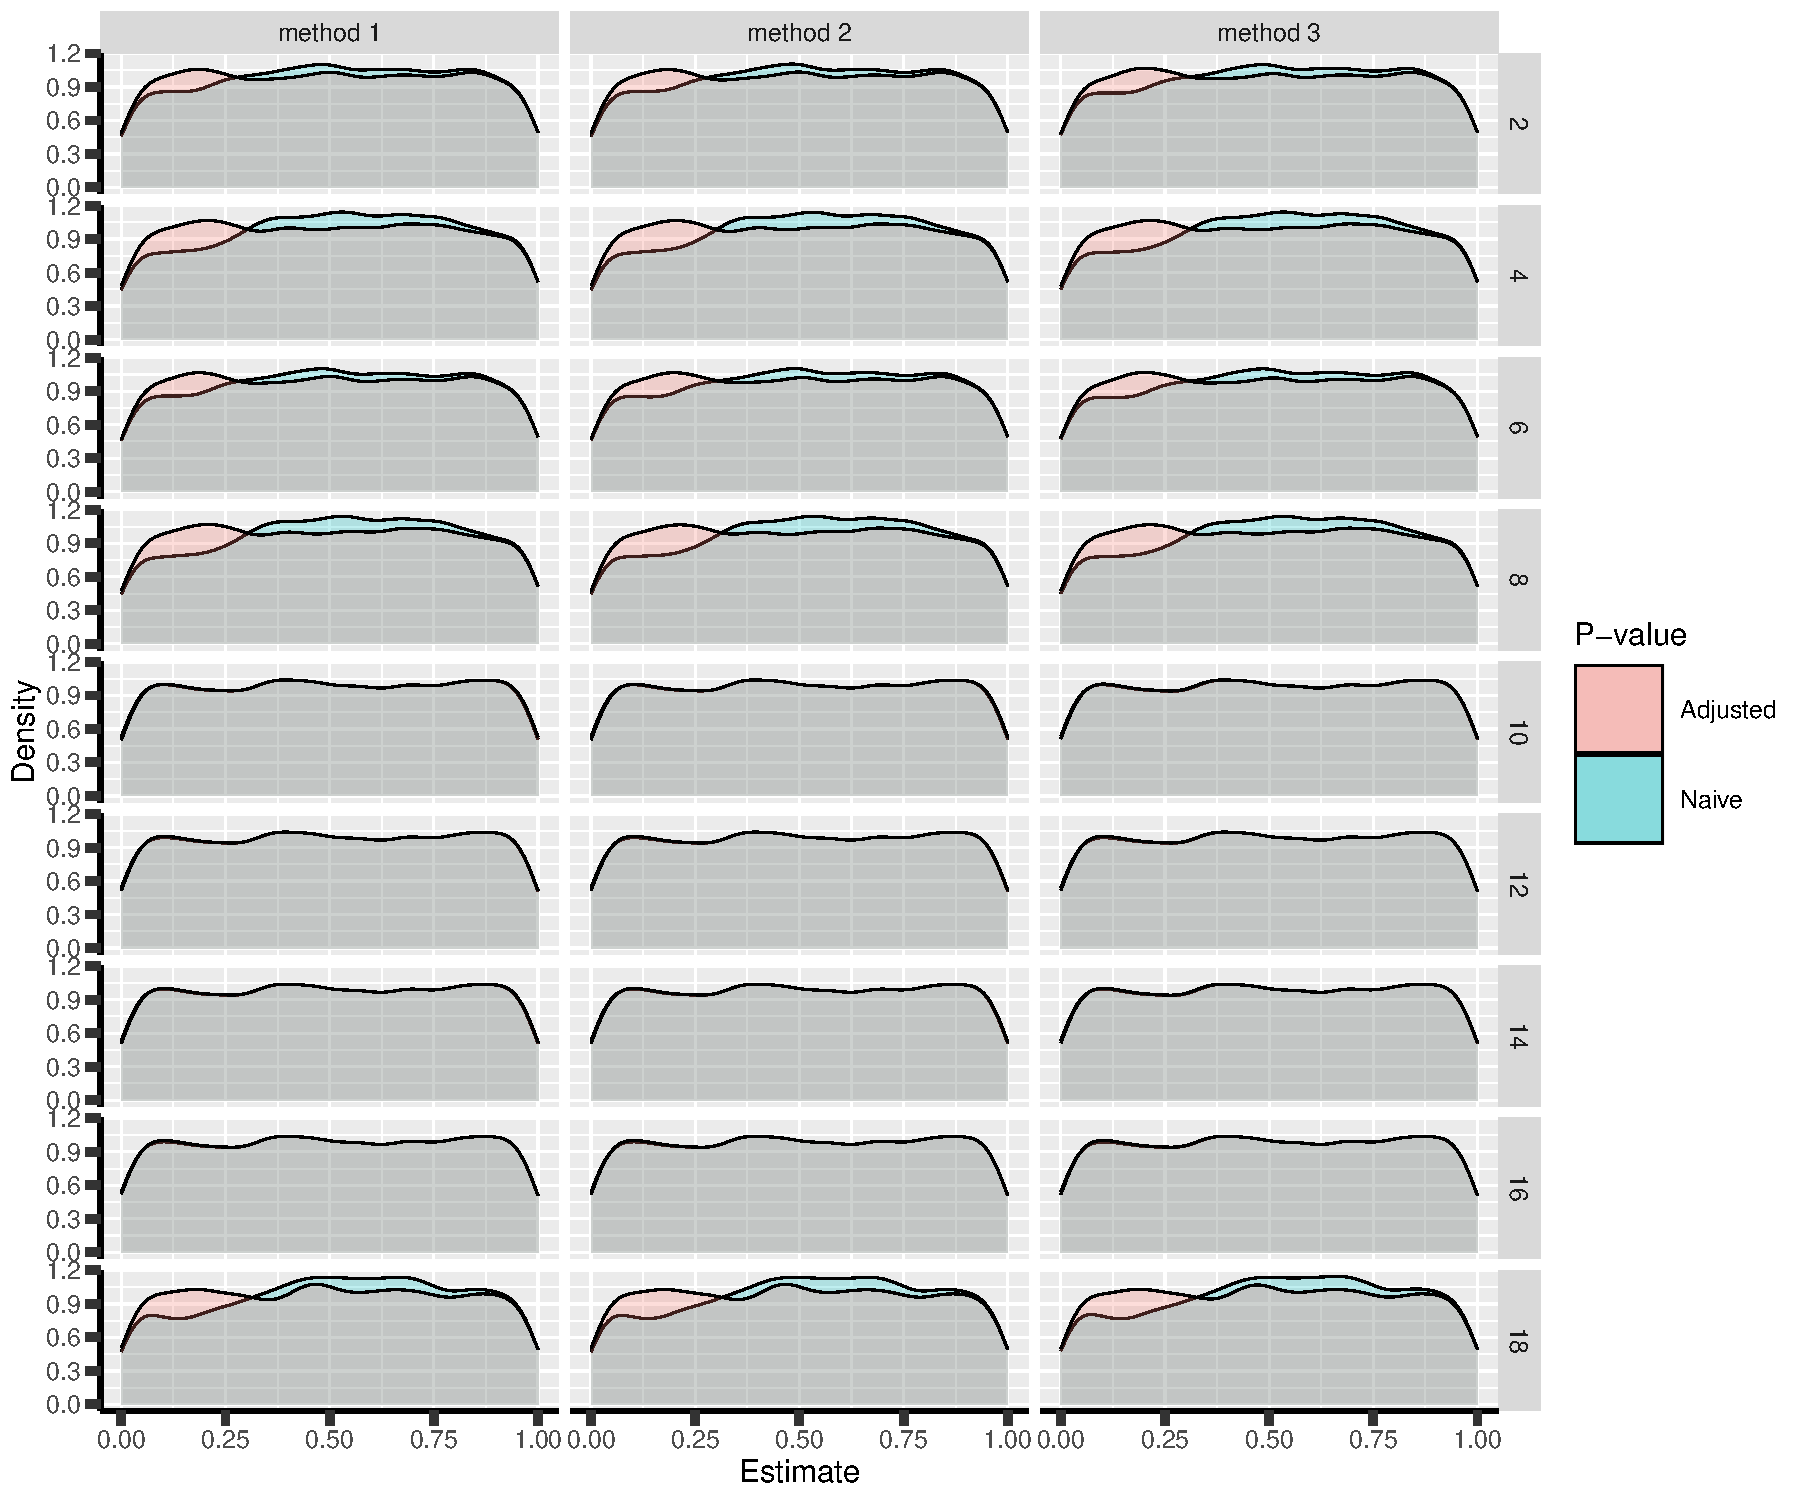
\includegraphics[trim={0 0 0 0},width=1\textwidth]{./figures/gg-pvalue-density.pdf}
\caption{Naive and adjusted p-value distribution over all simulations. Each row correspond to a different scenario}
\end{figure}

\clearpage

\section{Conclusion of the trial}
\label{sec:org6b2572b}

Relative frequency of stopping for efficacy/futility at decision/final

\begin{itemize}
\item Method 1
\end{itemize}
\begin{verbatim}
        N missing  hypo binding  fixC ar decision.eff decision.fut final.eff final.fut
 1: 10000    TRUE power    TRUE FALSE 10        37.82        6.050     43.18      13.0
 2: 10000    TRUE typeI    TRUE FALSE 10         0.79       70.850      1.67      26.7
 3: 10000    TRUE power    TRUE FALSE  5        35.60        6.020     45.00      13.4
 4: 10000    TRUE typeI    TRUE FALSE  5         0.68       69.210      1.74      28.4
 5: 10000    TRUE power    TRUE  TRUE 10        36.45        6.530     43.36      13.7
 6: 10000    TRUE typeI    TRUE  TRUE 10         0.64       71.290      1.61      26.5
 7: 10000    TRUE power    TRUE  TRUE  5        34.68        5.860     45.32      14.1
 8: 10000    TRUE typeI    TRUE  TRUE  5         0.72       69.110      1.70      28.5
 9: 10000    TRUE power   FALSE  TRUE 10        37.57        6.630     42.93      12.9
10:  2870    TRUE typeI   FALSE  TRUE 10         1.99        0.976      5.30      91.7
11: 10000    TRUE power   FALSE  TRUE  5        36.02        6.280     44.71      13.0
12:  3043    TRUE typeI   FALSE  TRUE  5         2.40        0.296      5.16      92.1
13: 10000    TRUE power   FALSE FALSE 10        38.32        5.870     42.35      13.5
14:  2874    TRUE typeI   FALSE FALSE 10         2.40        0.313      5.57      91.7
15: 10000    TRUE power   FALSE FALSE  5        36.75        5.700     43.90      13.6
16:  3080    TRUE typeI   FALSE FALSE  5         2.18        0.000      5.55      92.3
17: 10000   FALSE power    TRUE FALSE  5        33.98        5.330     46.33      14.4
18: 10000   FALSE typeI    TRUE FALSE  5         0.74       67.480      1.72      30.1
\end{verbatim}
\Warning something is not quite right for non-binding scenarios under the null (\texttt{N} should be 10000).

\clearpage

Method 2:
\begin{verbatim}
        N missing  hypo binding  fixC ar decision.eff decision.fut final.eff final.fut
 1: 10000    TRUE power    TRUE FALSE 10        37.66       6.2200     43.13      13.0
 2: 10000    TRUE typeI    TRUE FALSE 10         0.85      71.1800      1.68      26.3
 3: 10000    TRUE power    TRUE FALSE  5        35.55       6.1000     44.90      13.5
 4: 10000    TRUE typeI    TRUE FALSE  5         0.67      69.0500      1.74      28.5
 5: 10000    TRUE power    TRUE  TRUE 10        36.82       5.9400     43.59      13.6
 6: 10000    TRUE typeI    TRUE  TRUE 10         0.63      70.0200      1.62      27.7
 7: 10000    TRUE power    TRUE  TRUE  5        35.06       5.6300     45.40      13.9
 8: 10000    TRUE typeI    TRUE  TRUE  5         0.71      68.4600      1.68      29.1
 9: 10000    TRUE power   FALSE  TRUE 10        37.76       6.2100     43.09      12.9
10:  2956    TRUE typeI   FALSE  TRUE 10         1.89       0.8796      5.18      92.1
11: 10000    TRUE power   FALSE  TRUE  5        36.07       6.1000     44.75      13.1
12:  3093    TRUE typeI   FALSE  TRUE  5         2.33       0.2263      5.04      92.4
13: 10000    TRUE power   FALSE FALSE 10        38.33       6.1100     42.27      13.3
14:  2820    TRUE typeI   FALSE FALSE 10         2.45       0.3191      5.64      91.6
15: 10000    TRUE power   FALSE FALSE  5        36.78       5.7200     43.86      13.6
16:  3075    TRUE typeI   FALSE FALSE  5         2.15       0.0325      5.56      92.3
17: 10000   FALSE power    TRUE FALSE  5        33.68       5.1700     46.60      14.5
18: 10000   FALSE typeI    TRUE FALSE  5         0.72      67.4200      1.72      30.1
\end{verbatim}
\Warning something is not quite right for non-binding scenarios under the null (\texttt{N} should be 10000).

\clearpage

Method 3:
\begin{verbatim}
        N missing  hypo binding  fixC ar decision.eff decision.fut final.eff final.fut
 1: 10000    TRUE power    TRUE FALSE 10        40.44        6.540     40.01      13.0
 2: 10000    TRUE typeI    TRUE FALSE 10         0.74       68.770      1.66      28.8
 3: 10000    TRUE power    TRUE FALSE  5        36.49        6.420     43.72      13.4
 4: 10000    TRUE typeI    TRUE FALSE  5         0.68       68.370      1.72      29.2
 5: 10000    TRUE power    TRUE  TRUE 10        39.85        5.830     40.54      13.8
 6: 10000    TRUE typeI    TRUE  TRUE 10         0.73       68.890      1.72      28.7
 7: 10000    TRUE power    TRUE  TRUE  5        35.70        5.810     44.38      14.1
 8: 10000    TRUE typeI    TRUE  TRUE  5         0.78       68.260      1.72      29.2
 9: 10000    TRUE power   FALSE  TRUE 10        41.03        6.390     39.88      12.7
10:  3086    TRUE typeI   FALSE  TRUE 10         2.33        1.231      4.99      91.4
11: 10000    TRUE power   FALSE  TRUE  5        37.08        6.140     43.67      13.1
12:  3133    TRUE typeI   FALSE  TRUE  5         2.36        0.447      5.08      92.1
13: 10000    TRUE power   FALSE FALSE 10        41.47        6.050     39.18      13.3
14:  3130    TRUE typeI   FALSE FALSE 10         2.59        0.990      5.27      91.2
15: 10000    TRUE power   FALSE FALSE  5        37.37        5.860     43.09      13.7
16:  3163    TRUE typeI   FALSE FALSE  5         2.37        0.253      5.41      92.0
17: 10000   FALSE power    TRUE FALSE  5        34.66        5.580     45.27      14.5
18: 10000   FALSE typeI    TRUE FALSE  5         0.68       66.540      1.77      31.0
\end{verbatim}
\Warning something is not quite right for non-binding scenarios under the null (\texttt{N} should be 10000).

\clearpage

\section{Bias (True effect: 0.6 under the alternative)}
\label{sec:org98258a3}

\bigskip

Bias \footnote{average difference between the estimate and the truth} per estimator and method:
\begin{adjustwidth}{-1cm}{-1cm}
\begin{verbatim}
     hypo missing binding  fixC ar biasMLE1 biasMLE2 biasMLE3 biasMUE1 biasMUE2 biasMUE3
 1: power    TRUE    TRUE FALSE 10   0.0130   0.0131   0.0141  0.00547  0.00556  0.00321
 2: typeI    TRUE    TRUE FALSE 10  -0.0184  -0.0184  -0.0185 -0.00426 -0.00433 -0.00472
 3: power    TRUE    TRUE FALSE  5   0.0224   0.0222   0.0234  0.01008  0.01016  0.00902
 4: typeI    TRUE    TRUE FALSE  5  -0.0304  -0.0308  -0.0306 -0.01176 -0.01214 -0.01214
 5: power    TRUE    TRUE  TRUE 10   0.0116   0.0121   0.0130  0.00457  0.00504  0.00306
 6: typeI    TRUE    TRUE  TRUE 10  -0.0221  -0.0223  -0.0223 -0.00817 -0.00830 -0.00816
 7: power    TRUE    TRUE  TRUE  5   0.0216   0.0220   0.0227  0.00990  0.01050  0.00875
 8: typeI    TRUE    TRUE  TRUE  5  -0.0339  -0.0344  -0.0341 -0.01450 -0.01457 -0.01499
 9: power    TRUE   FALSE  TRUE 10   0.0150   0.0151   0.0163  0.00371  0.00376  0.00221
10: typeI    TRUE   FALSE  TRUE 10   0.1776   0.1740   0.1713  0.17905  0.17536  0.17171
11: power    TRUE   FALSE  TRUE  5   0.0242   0.0242   0.0252  0.00864  0.00835  0.00797
12: typeI    TRUE   FALSE  TRUE  5   0.1722   0.1701   0.1700  0.17292  0.17079  0.16962
13: power    TRUE   FALSE FALSE 10   0.0144   0.0141   0.0157  0.00338  0.00297  0.00317
14: typeI    TRUE   FALSE FALSE 10   0.1803   0.1821   0.1736  0.18129  0.18315  0.17484
15: power    TRUE   FALSE FALSE  5   0.0234   0.0233   0.0243  0.00884  0.00883  0.00811
16: typeI    TRUE   FALSE FALSE  5   0.1721   0.1720   0.1705  0.17225  0.17208  0.17059
17: power   FALSE    TRUE FALSE  5   0.0228   0.0228   0.0238  0.01197  0.01208  0.01063
18: typeI   FALSE    TRUE FALSE  5  -0.0295  -0.0297  -0.0299 -0.01105 -0.01139 -0.01161
\end{verbatim}
\end{adjustwidth}
\Warning clear bias for non-binding scenarios under the null

Median bias \footnote{Relative frequency at which the estimate is greater than the truth minus 0.5} per estimator and method:
\begin{adjustwidth}{-1cm}{-1cm}
\begin{verbatim}
     hypo missing binding  fixC ar mbiasMLE1 mbiasMLE2 mbiasMLE3 mbiasMUE1 mbiasMUE2 mbiasMUE3
 1: power    TRUE    TRUE FALSE 10    0.0250    0.0240    0.0266   -0.0023   -0.0017   -0.0042
 2: typeI    TRUE    TRUE FALSE 10   -0.0193   -0.0198   -0.0223    0.0002   -0.0013    0.0001
 3: power    TRUE    TRUE FALSE  5    0.0387    0.0382    0.0406   -0.0030   -0.0016   -0.0018
 4: typeI    TRUE    TRUE FALSE  5   -0.0346   -0.0339   -0.0361    0.0000   -0.0002    0.0001
 5: power    TRUE    TRUE  TRUE 10    0.0164    0.0188    0.0179   -0.0053   -0.0061   -0.0080
 6: typeI    TRUE    TRUE  TRUE 10   -0.0327   -0.0314   -0.0347   -0.0113   -0.0079   -0.0099
 7: power    TRUE    TRUE  TRUE  5    0.0356    0.0369    0.0361   -0.0073   -0.0075   -0.0075
 8: typeI    TRUE    TRUE  TRUE  5   -0.0473   -0.0492   -0.0493   -0.0105   -0.0081   -0.0105
 9: power    TRUE   FALSE  TRUE 10    0.0328    0.0301    0.0345   -0.0025   -0.0044   -0.0036
10: typeI    TRUE   FALSE  TRUE 10    0.3599    0.3555    0.3474    0.3606    0.3562    0.3487
11: power    TRUE   FALSE  TRUE  5    0.0479    0.0459    0.0499   -0.0014   -0.0012   -0.0026
12: typeI    TRUE   FALSE  TRUE  5    0.3413    0.3432    0.3379    0.3413    0.3432    0.3382
13: power    TRUE   FALSE FALSE 10    0.0326    0.0324    0.0339   -0.0033   -0.0036    0.0012
14: typeI    TRUE   FALSE FALSE 10    0.3605    0.3621    0.3482    0.3612    0.3628    0.3508
15: power    TRUE   FALSE FALSE  5    0.0442    0.0442    0.0465   -0.0010   -0.0010   -0.0028
16: typeI    TRUE   FALSE FALSE  5    0.3455    0.3452    0.3410    0.3455    0.3452    0.3416
17: power   FALSE    TRUE FALSE  5    0.0383    0.0378    0.0400   -0.0026   -0.0008   -0.0038
18: typeI   FALSE    TRUE FALSE  5   -0.0329   -0.0336   -0.0353    0.0044    0.0031    0.0035
\end{verbatim}

\end{adjustwidth}

\clearpage

\section{Distribution of the estimates}
\label{sec:org0a985ba}

Distribution of the estimates:
\begin{figure}[!h]
\centering
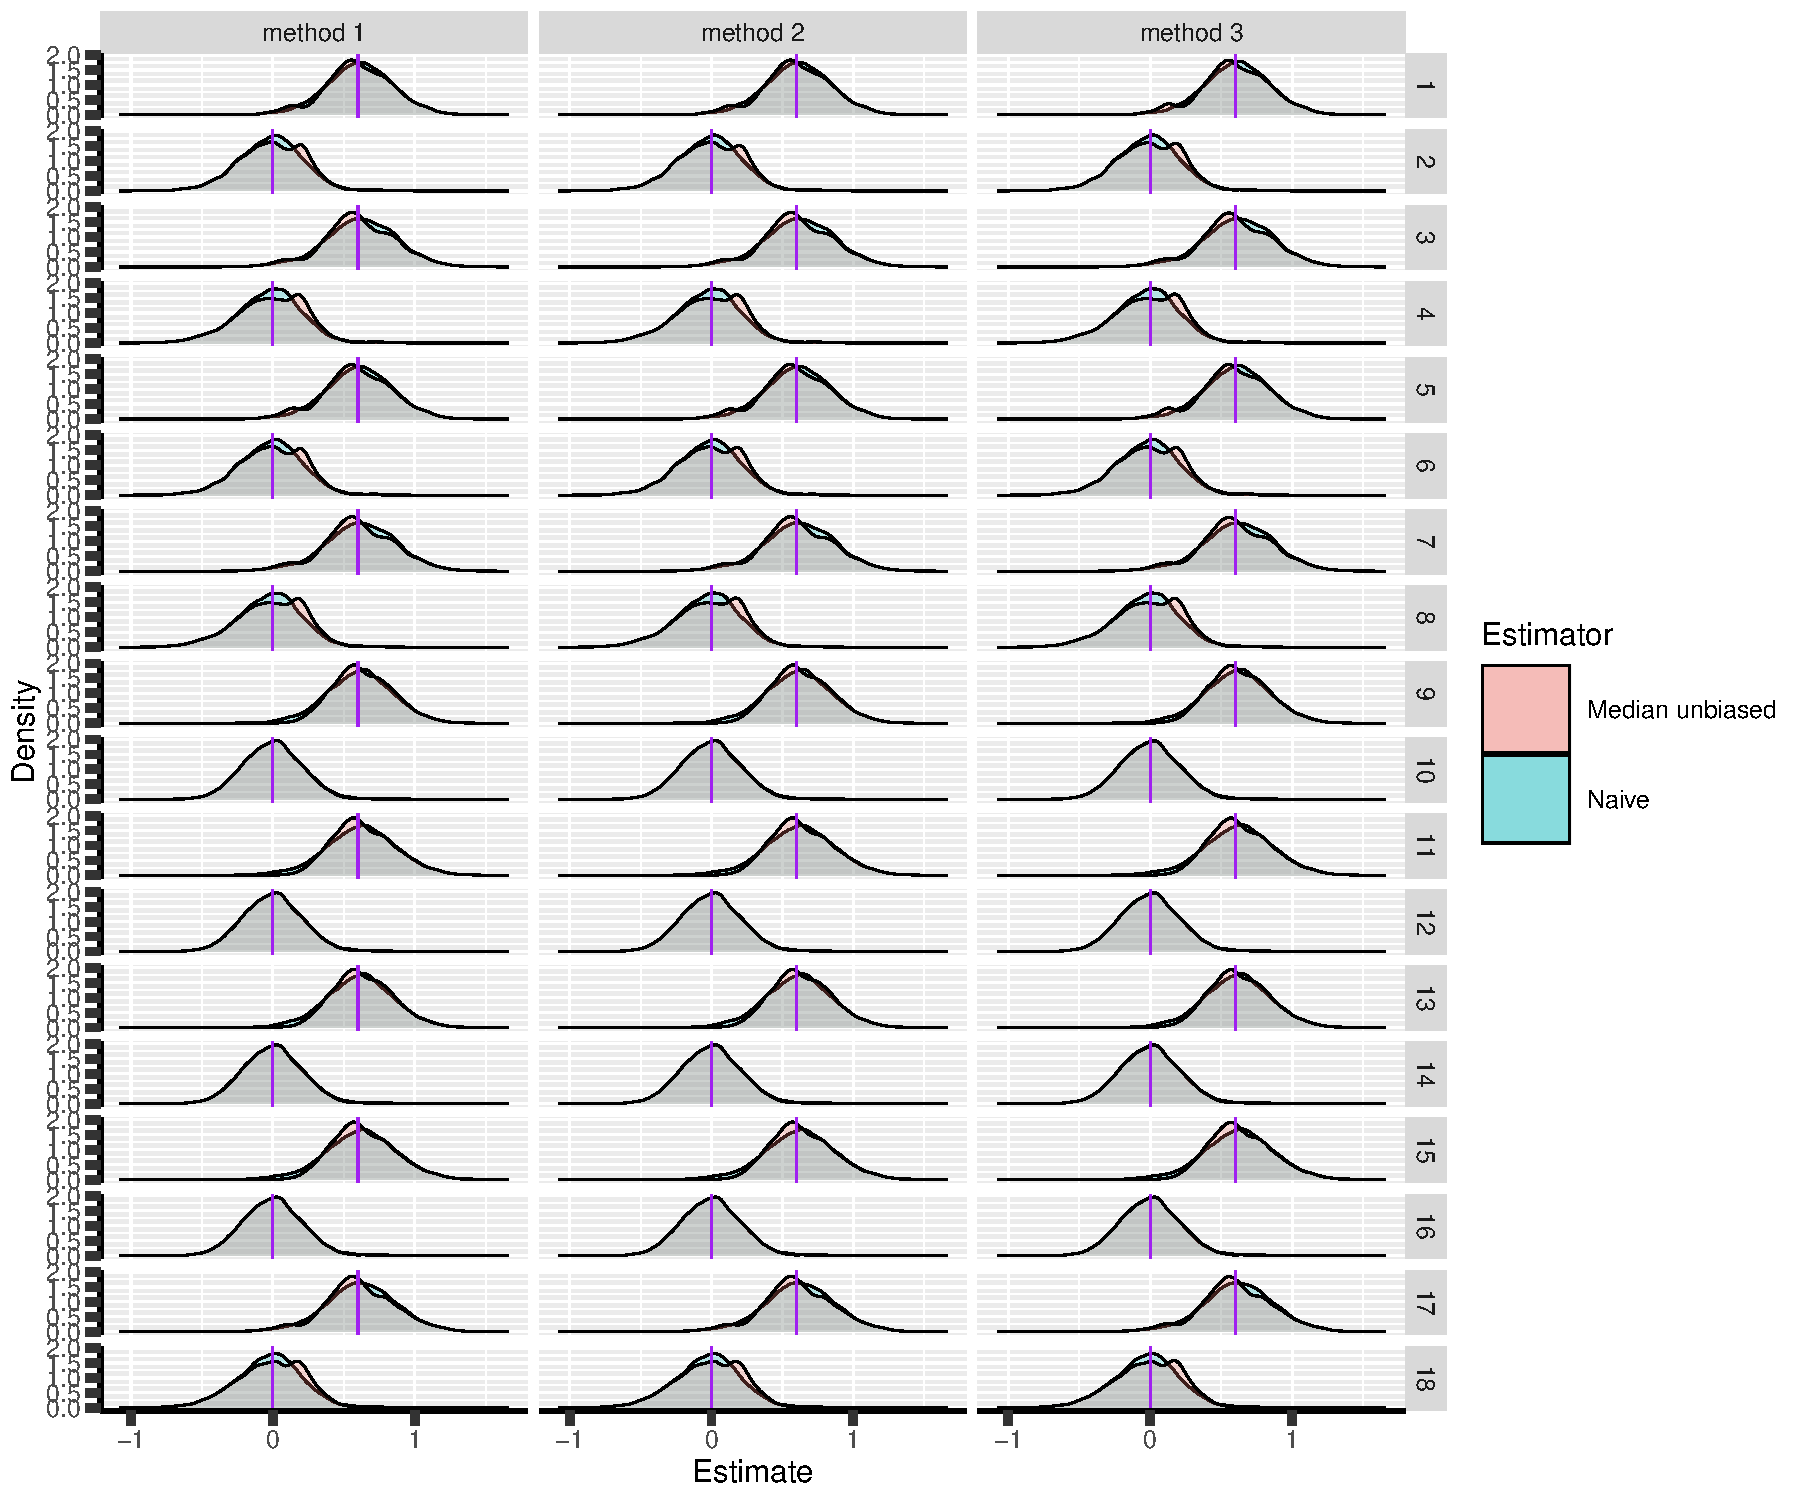
\includegraphics[trim={0 0 0 0},width=1\textwidth]{./figures/gg-estimate-density.pdf}
\caption{Naive and Median unbiased estimate distribution over all simulations. Each row correspond to a different scenario}
\end{figure}

\begin{figure}[!h]
\centering
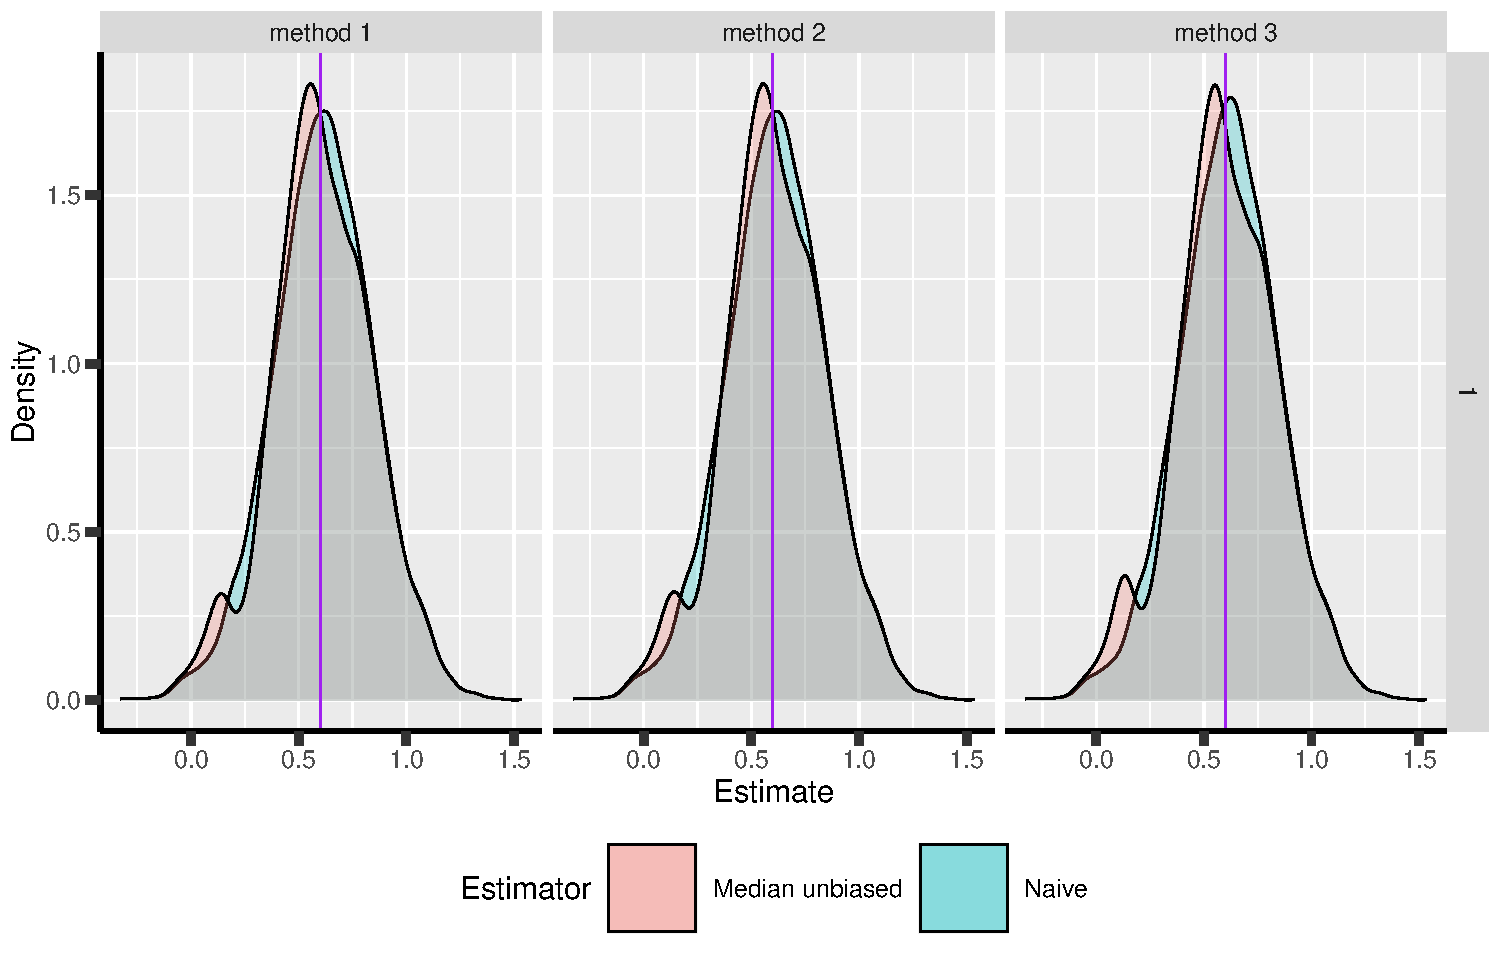
\includegraphics[trim={0 0 0 0},width=0.8\textwidth]{./figures/gg-estimate-density-scenario1.pdf}
\caption{Same but specific to scenario 1}
\end{figure}

\clearpage

Distribution of the median unbiased estimate conditional to the stage:
\begin{figure}[!h]
\centering
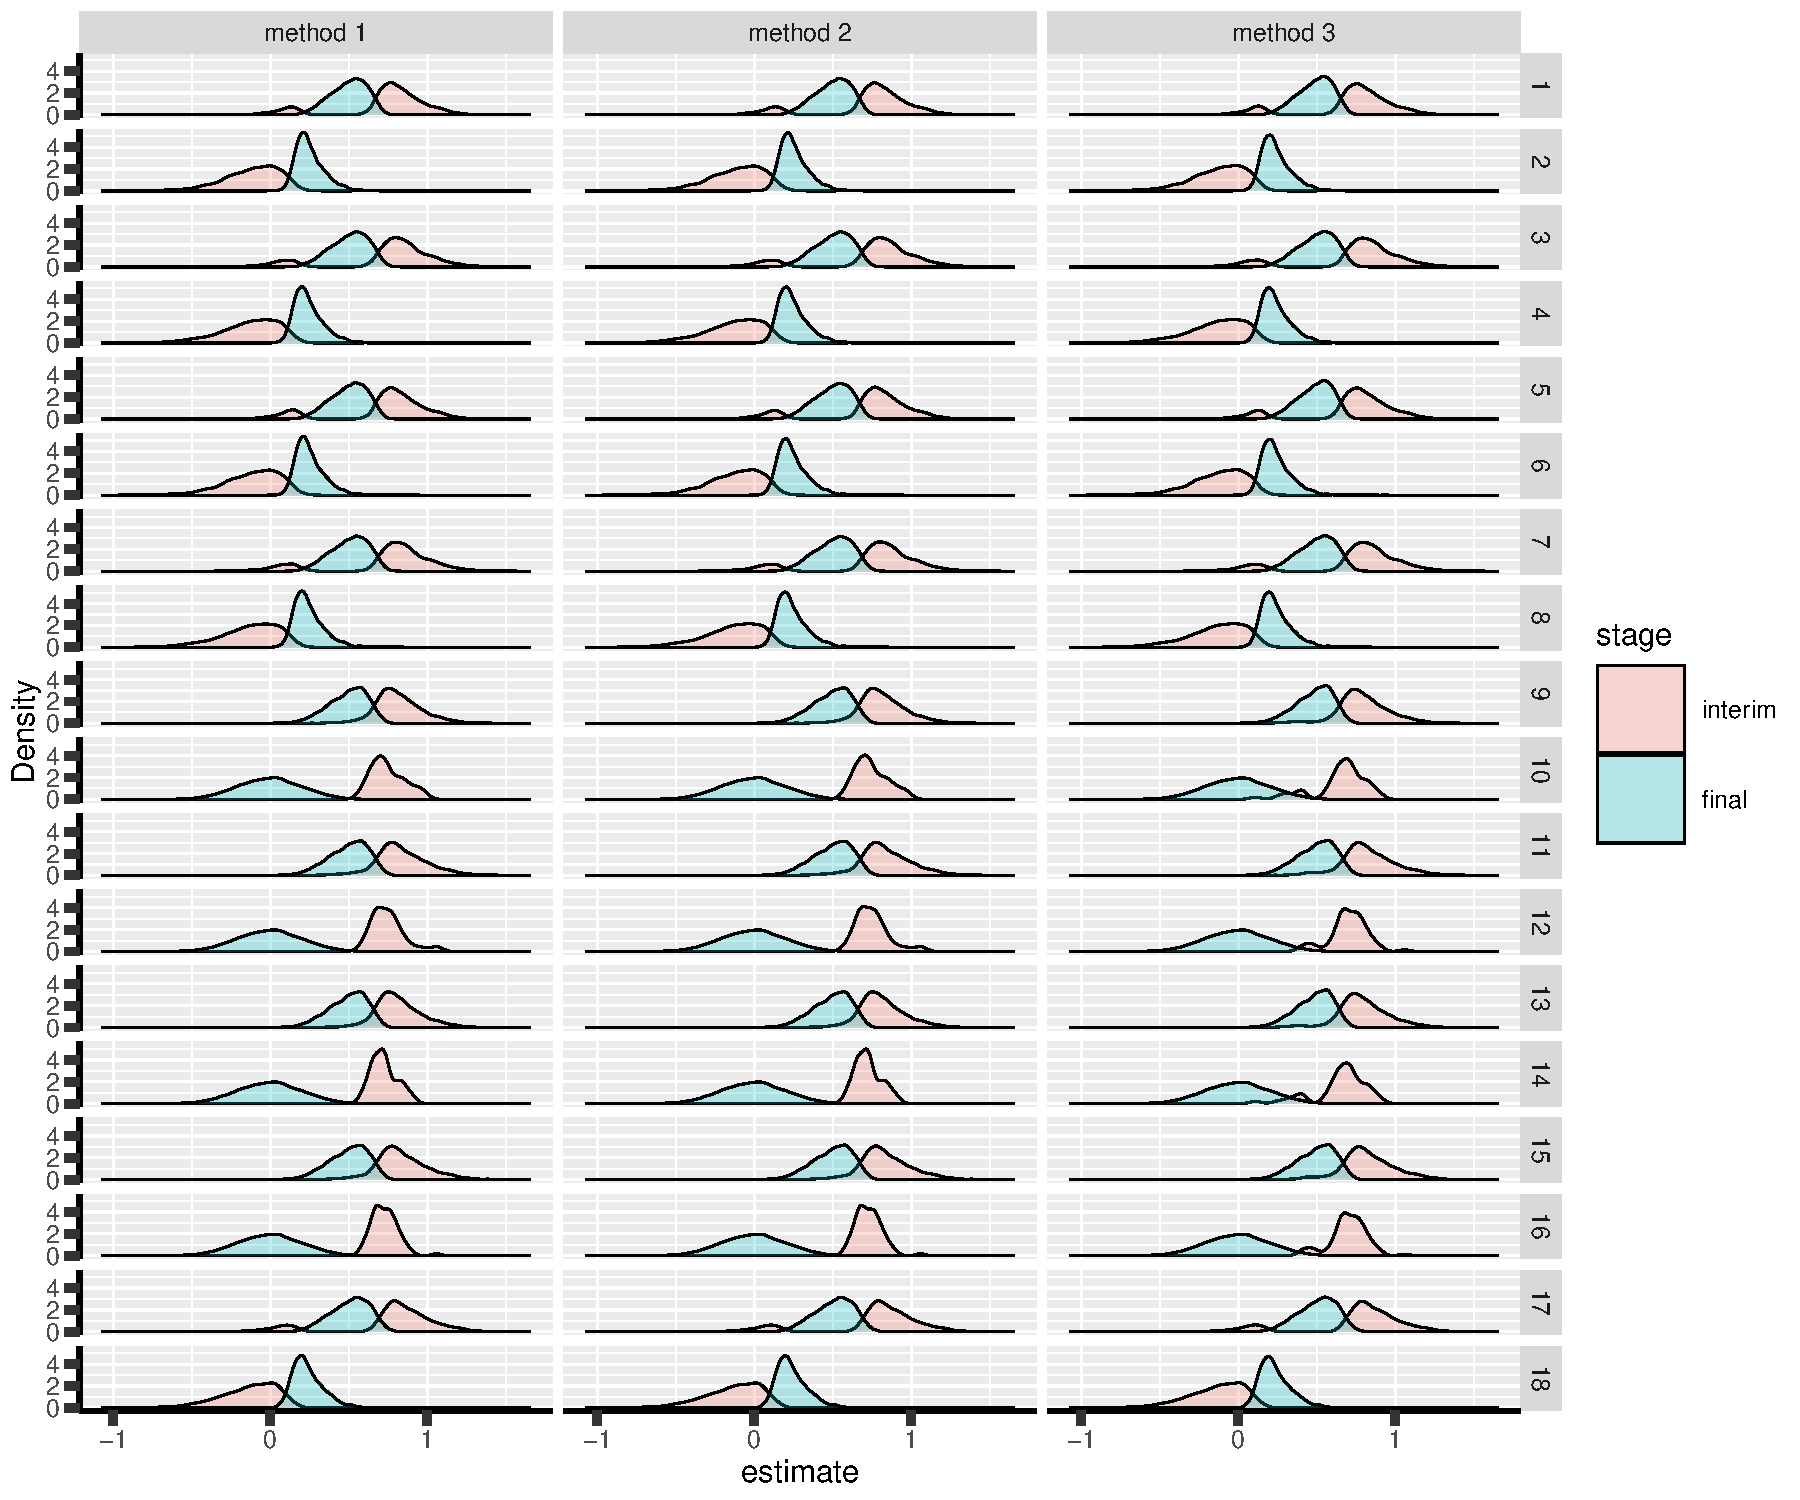
\includegraphics[trim={0 0 0 0},width=1\textwidth]{./figures/gg-estimateC-density.pdf}
\caption{Median unbiased estimate distribution conditional to the stage. Each row correspond to a different scenario.}
\end{figure}

\clearpage

\section{Special cases}
\label{sec:org3eb8c71}

Reason for stopping (first 4) or continuing the trial (last):
\begin{verbatim}
                              scenario    1    2    3    4    5    6    7    8
reason                 method                                                 
decreasing information 1                  0    0    1    1    0    0    0    0
                       2                  0    0    1    1    0    0    0    0
                       3                  0    0    1    1    0    0    0    0
efficacy               1               3740   77 3559   67 3696   82 3502   82
                       2               3729   82 3554   68 3732   82 3546   83
                       3               4137  107 3712   83 4071  110 3632   92
futility               1                646 7086  603 6922  600 7109  552 6901
                       2                658 7120  611 6904  542 6981  523 6834
                       3                560 6843  579 6822  495 6850  519 6812
Imax reached           1                  1    1    0    0    2    2    0    0
                       2                  1    1    0    0    2    2    0    0
                       3                  1    1    0    0    2    2    0    0
no boundary crossed    1               5613 2836 5838 3011 5702 2807 5946 3017
                       2               5612 2797 5835 3028 5724 2935 5931 3083
                       3               5302 3049 5709 3095 5432 3038 5849 3096
\end{verbatim}

\begin{verbatim}
                              scenario    9   10   11   12   13   14   15   16
reason                 method                                                 
decreasing information 1                  0    0    1    0    0    0    0    0
                       2                  0    0    1    0    0    0    0    0
                       3                  0    0    1    0    0    0    0    0
efficacy               1               3805   84 3634   82 3815   78 3674   67
                       2               3824   81 3646   79 3816   78 3677   67
                       3               4206  109 3761   88 4238  112 3788   83
futility               1                614 7130  596 6957  604 7126  571 6920
                       2                572 7044  571 6907  628 7180  573 6925
                       3                535 6914  561 6867  514 6870  535 6837
Imax reached           1                  1    1    0    0    0    0    0    0
                       2                  1    1    0    0    0    0    0    0
                       3                  1    1    0    0    0    0    0    0
no boundary crossed    1               5580 2785 5770 2961 5581 2796 5755 3013
                       2               5603 2874 5783 3014 5556 2742 5750 3008
                       3               5258 2976 5678 3045 5248 3018 5677 3080
\end{verbatim}

\clearpage

\section{Reversal probability}
\label{sec:org238ee19}

Percentage of time we observe a reversal:
\begin{adjustwidth}{-1cm}{-1cm}
\begin{verbatim}
        N  hypo missing ar binding  fixC fu2eff_1 fu2eff_2 fu2eff_3 eff2fu_1 eff2fu_2 eff2fu_3
 1: 10000 power   FALSE  5    TRUE FALSE     0.06     0.07     0.01     0.04     0.04     0.63
 2: 10000 power    TRUE  5   FALSE FALSE     0.04     0.04     0.00     0.03     0.03     0.51
 3: 10000 power    TRUE  5   FALSE  TRUE     0.04     0.03     0.03     0.36     0.42     0.56
 4: 10000 power    TRUE  5    TRUE FALSE     0.06     0.08     0.02     0.05     0.07     0.65
 5: 10000 power    TRUE  5    TRUE  TRUE     0.02     0.02     0.01     0.36     0.42     0.63
 6: 10000 power    TRUE 10   FALSE FALSE     0.35     0.38     0.05     0.18     0.21     0.96
 7: 10000 power    TRUE 10   FALSE  TRUE     0.15     0.13     0.10     0.63     0.61     1.13
 8: 10000 power    TRUE 10    TRUE FALSE     0.57     0.57     0.13     0.15     0.20     1.06
 9: 10000 power    TRUE 10    TRUE  TRUE     0.17     0.16     0.11     0.70     0.68     0.99
10: 10000 typeI   FALSE  5    TRUE FALSE     0.01     0.03     0.00     0.01     0.03     0.12
11: 10000 typeI    TRUE  5   FALSE FALSE     0.00     0.00     0.00     0.00     0.01     0.08
12: 10000 typeI    TRUE  5   FALSE  TRUE     0.00     0.00     0.00     0.09     0.07     0.14
13: 10000 typeI    TRUE  5    TRUE FALSE     0.02     0.02     0.00     0.01     0.03     0.15
14: 10000 typeI    TRUE  5    TRUE  TRUE     0.00     0.00     0.00     0.10     0.12     0.14
15: 10000 typeI    TRUE 10   FALSE FALSE     0.00     0.00     0.00     0.09     0.09     0.31
16: 10000 typeI    TRUE 10   FALSE  TRUE     0.00     0.00     0.00     0.27     0.25     0.37
17: 10000 typeI    TRUE 10    TRUE FALSE     0.11     0.11     0.03     0.09     0.08     0.36
18: 10000 typeI    TRUE 10    TRUE  TRUE     0.02     0.00     0.00     0.22     0.21     0.39
\end{verbatim}

\end{adjustwidth}


\clearpage

\section{Frequency mismatch p-value / boundaries}
\label{sec:orga257f0b}

When concluding for futility:
\begin{verbatim}
     hypo missing ar binding  fixC   method 1   method 2   method 3
 1: power   FALSE  5    TRUE FALSE 0.00000000 0.00000000 0.39860488
 2: power    TRUE  5   FALSE FALSE 0.41343669 0.41322314 0.46059365
 3: power    TRUE  5   FALSE  TRUE 1.92008303 2.29405631 0.41558442
 4: power    TRUE  5    TRUE FALSE 0.00000000 0.00000000 0.45477514
 5: power    TRUE  5    TRUE  TRUE 1.65000000 1.99590583 0.40160643
 6: power    TRUE 10   FALSE FALSE 2.43145370 2.47422680 0.93023256
 7: power    TRUE 10   FALSE  TRUE 5.23076923 4.75195822 1.15243583
 8: power    TRUE 10    TRUE FALSE 0.00000000 0.00000000 1.22762148
 9: power    TRUE 10    TRUE  TRUE 4.11094601 3.57325166 1.12187659
10: typeI   FALSE  5    TRUE FALSE 0.00000000 0.00000000 0.00000000
11: typeI    TRUE  5   FALSE FALSE 0.07037298 0.07047216 0.03428180
12: typeI    TRUE  5   FALSE  TRUE 0.31994312 0.24432810 0.03448276
13: typeI    TRUE  5    TRUE FALSE 0.00000000 0.00000000 0.02049180
14: typeI    TRUE  5    TRUE  TRUE 0.08198401 0.10244852 0.03076923
15: typeI    TRUE 10   FALSE FALSE 0.52930057 0.54012346 0.13869626
16: typeI    TRUE 10   FALSE  TRUE 0.75159714 0.69166363 0.00000000
17: typeI    TRUE 10    TRUE FALSE 0.00000000 0.00000000 0.04098361
18: typeI    TRUE 10    TRUE  TRUE 0.17391304 0.15345269 0.08200923
\end{verbatim}

When concluding for efficacy:
\begin{verbatim}
     hypo missing ar binding  fixC method 1 method 2 method 3
 1: power   FALSE  5    TRUE FALSE        0        0        0
 2: power    TRUE  5   FALSE FALSE        0        0        0
 3: power    TRUE  5   FALSE  TRUE        0        0        0
 4: power    TRUE  5    TRUE FALSE        0        0        0
 5: power    TRUE  5    TRUE  TRUE        0        0        0
 6: power    TRUE 10   FALSE FALSE        0        0        0
 7: power    TRUE 10   FALSE  TRUE        0        0        0
 8: power    TRUE 10    TRUE FALSE        0        0        0
 9: power    TRUE 10    TRUE  TRUE        0        0        0
10: typeI   FALSE  5    TRUE FALSE        0        0        0
11: typeI    TRUE  5   FALSE FALSE        0        0        0
12: typeI    TRUE  5   FALSE  TRUE        0        0        0
13: typeI    TRUE  5    TRUE FALSE        0        0        0
14: typeI    TRUE  5    TRUE  TRUE        0        0        0
15: typeI    TRUE 10   FALSE FALSE        0        0        0
16: typeI    TRUE 10   FALSE  TRUE        0        0        0
17: typeI    TRUE 10    TRUE FALSE        0        0        0
18: typeI    TRUE 10    TRUE  TRUE        0        0        0
\end{verbatim}

\clearpage

\section{Percentage of missing values}
\label{sec:org2661dcd}

Here only for method 1 - values are very similar between different
methods:
\begin{itemize}
\item \texttt{pc.all} percentage of observations with full data
\item \texttt{pc.missing3} percentage of observations missing the final outcome
but with intermediate outcome value and baseline.
\item \texttt{pc.missing23} percentage of observations with only baseline value
\end{itemize}
\begin{verbatim}
    method missing ar  hypo  fixC binding     N   pc.all pc.missing3 pc.missing23
 1:      1    TRUE  5 power FALSE    TRUE 10000 79.53472    9.562374    10.902910
 2:      1    TRUE  5 typeI FALSE    TRUE 10000 79.53472    9.562374    10.902910
 3:      1    TRUE  5 power  TRUE    TRUE 10000 79.44022    9.531225    11.028558
 4:      1    TRUE  5 typeI  TRUE    TRUE 10000 79.44022    9.531225    11.028558
 5:      1    TRUE  5 power  TRUE   FALSE 10000 79.71917    9.427430    10.853396
 6:      1    TRUE  5 typeI  TRUE   FALSE 10000 79.71917    9.427430    10.853396
 7:      1    TRUE  5 power FALSE   FALSE 10000 79.64196    9.449136    10.908902
 8:      1    TRUE  5 typeI FALSE   FALSE 10000 79.64196    9.449136    10.908902
 9:      1   FALSE  5 power FALSE    TRUE 10000 87.78863    6.090240     6.121126
10:      1   FALSE  5 typeI FALSE    TRUE 10000 87.78863    6.090240     6.121126
11:      1    TRUE 10 power FALSE    TRUE 10000 71.60971   13.327969    15.062319
12:      1    TRUE 10 typeI FALSE    TRUE 10000 71.60971   13.327969    15.062319
13:      1    TRUE 10 power  TRUE    TRUE 10000 71.52189   13.282615    15.195496
14:      1    TRUE 10 typeI  TRUE    TRUE 10000 71.52189   13.282615    15.195496
15:      1    TRUE 10 power  TRUE   FALSE 10000 71.85935   13.144488    14.996166
16:      1    TRUE 10 typeI  TRUE   FALSE 10000 71.85935   13.144488    14.996166
17:      1    TRUE 10 power FALSE   FALSE 10000 71.79364   13.168843    15.037522
18:      1    TRUE 10 typeI FALSE   FALSE 10000 71.79364   13.168843    15.037522
\end{verbatim}

\clearpage

\section{Information}
\label{sec:orgd6ef13b}

Percentage of information for method 1\footnote{average over the reached stages}:
\begin{verbatim}
 scenario missing binding  fixC ar  interim decision     final
        1    TRUE    TRUE FALSE 10 54.56262 63.87624 102.43196
        2    TRUE    TRUE FALSE 10 54.56262 68.44170 102.27378
        3    TRUE    TRUE FALSE  5 53.19699 57.43534 102.53302
        4    TRUE    TRUE FALSE  5 53.19699 60.05461 102.25032
        5    TRUE    TRUE  TRUE 10 54.46422 63.55543 102.55590
        6    TRUE    TRUE  TRUE 10 54.46422 68.38828 102.04570
        7    TRUE    TRUE  TRUE  5 53.10347 57.19873 102.61372
        8    TRUE    TRUE  TRUE  5 53.10347 59.95959 102.13328
        9    TRUE   FALSE  TRUE 10 54.52041 63.81588 102.45701
       10    TRUE   FALSE  TRUE 10 54.52041 68.36137 102.14337
       11    TRUE   FALSE  TRUE  5 53.18289 57.37841 102.60304
       12    TRUE   FALSE  TRUE  5 53.18289 60.00160 102.25444
       13    TRUE   FALSE FALSE 10 54.50746 63.85073 102.45852
       14    TRUE   FALSE FALSE 10 54.50746 68.22472 102.26402
       15    TRUE   FALSE FALSE  5 53.16583 57.37762 102.59683
       16    TRUE   FALSE FALSE  5 53.16583 59.91894 102.19314
       17   FALSE    TRUE FALSE  5 51.99597 56.30990  99.79909
       18   FALSE    TRUE FALSE  5 51.99597 59.23342  99.51892
\end{verbatim}

Similar results for other methods.
\end{document}